\newpage




\section{Automaton}\label{sec:automaton} 
 
 

\begin{figure}[h]
    \centering
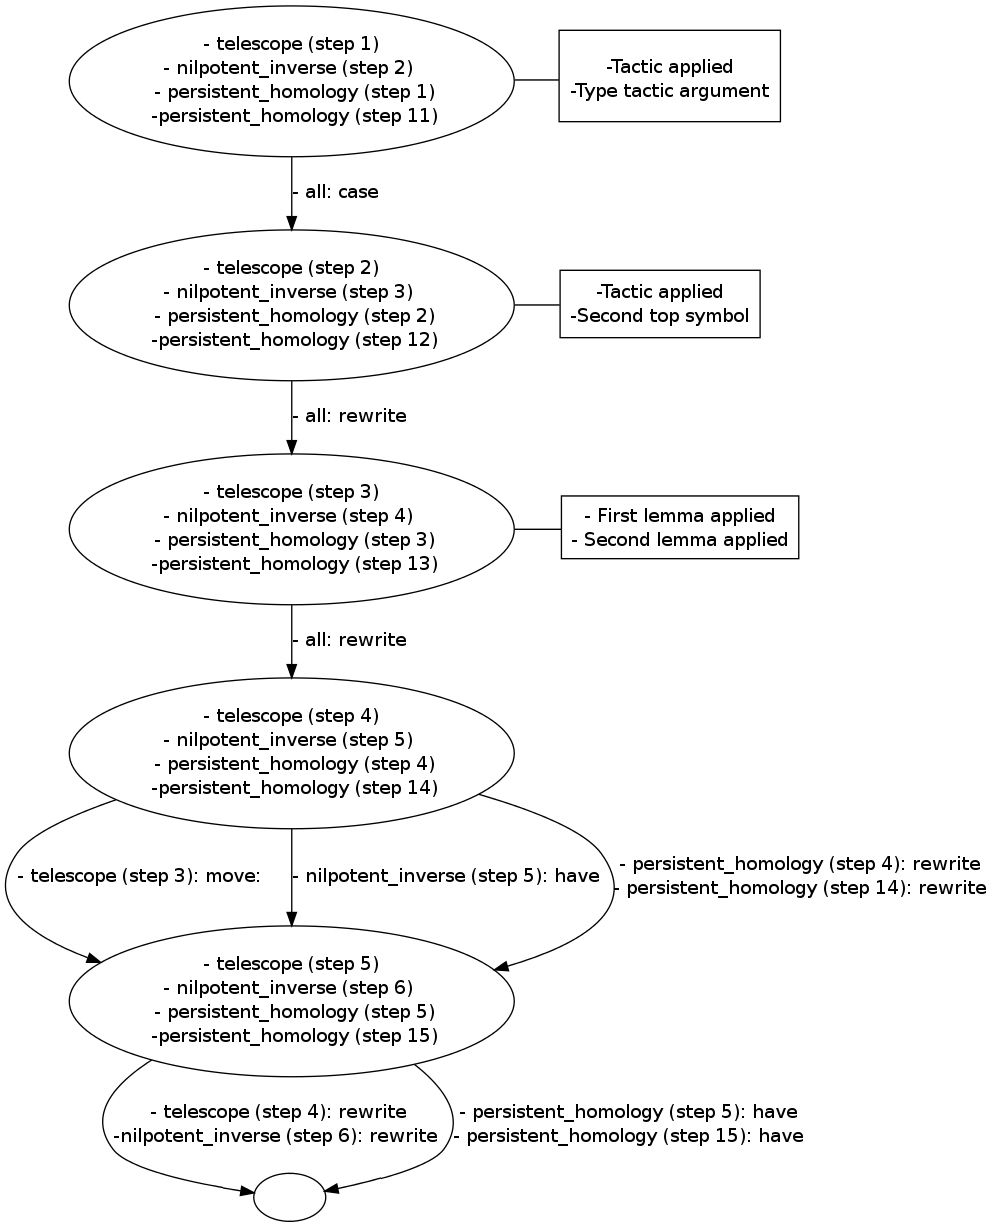
\includegraphics[scale=0.28]{itp.png} 
\caption{\scriptsize{\emph{Automaton corresponding to the proof cluster of four lemma fragments described in the case study of Section~\ref{sec:recurrent}.} The automaton shows the five proof steps, of which the first three are shown to influence the cluster formation.
It uses Lemma names: \texttt{telescope} for the lemma of Example~\ref{example0}, \texttt{nilpotent\_inverse} for Lemma~\ref{lem:nilpotent2}, and \texttt{persistent\_homology} 
for Lemma~\ref{lem:fundamental}.
  In addition to Lemma names, ML4PG can show lemma statements, and it can provide details of the \lq\lq{}Tactic applied\rq\rq{}, \lq\lq{}Type tactic argument\rq\rq{}, \lq\lq{}Second top symbol\rq\rq{}, \lq\lq{}First/Second lemma applied\rq\rq{} fields.}}
\end{figure}




